\section{Experimentaci\'on} \label{section:Experimentation}

Con el objetivo de comprobar la viabilidad y funcionamiento del prototipo implementado se propone la evaluaci\'on 
de su comportamiento ante dos escenarios de prueba. A continuaci\'on se describen los detalles de los experimentos.

\subsection{Ambiente de experimentaci\'on}

\subsubsection{Equipo}

Se utilizó una computadora portátil con un procesador Intel(R) Core(TM) i7-11370H 11th Gen @ 3.30GHz, 16GB de 
memoria RAM y sistema operativo Windows 11 Home 23H2.

\subsubsection{Docker}

Se utilizó Docker para simular el traspaso de datos por red entre la aplicaci\'on, el Cat\'alogo de Datos y 
los servidores de bases de datos fuente y destino. Se crea una im\'agen de la aplicaci\'on basada en python:3.10, con el 
nombre \textbf{autoetl}. 
Con el archivo \textbf{docker-compose.yml} se inicializan todos los contenedores que intervienen en el proceso 
de experimentaci\'on. Los servidores de bases de datos fuente y destino son contenedores de PostgreSQL llamados 
\textbf{db} y \textbf{target} respectivamente. El Cat\'alogo de Datos es un contenedor de Neo4j con nombre 
\textbf{data\_catalog}. La aplicaci\'on implementada yace en un contenedor de la imagen creada \textbf{autoetl}. 
Por \'ultimo, con el objetivo de visualizar los resultados del proceso de poblaci\'on se añade al ambiente un 
contenedor de \textbf{pgadmin4}, el cual proporciona una herramienta para la visualizaci\'on de bases de datos 
de PostgreSQL.




Con el objetivo de validar la solución propuesta, se ha desarrollado un sistema transaccional que registra las 
ventas de una red de tiendas minoristas. Este escenario se basa en \textbf{Retail Sales} expuesto en el Cap\'itulo 2
de \cite{kimball2011data}. A continuación, se detalla el caso de estudio:

La red de tiendas cuenta con sucursales distribuidas en varias provincias del país. Estas tiendas se encuentran ubicadas 
en diferentes barrios de los municipios de cada provincia. Para cada provincia, se registra su nombre, mientras que para 
cada municipio se almacena tanto su nombre como la provincia a la que pertenece. Asimismo, se guarda el nombre y el 
municipio al que pertenece cada barrio donde se encuentran las tiendas.

Cada tienda tiene un nombre específico y está situada en un barrio en particular. Todas las tiendas comparten una serie 
de departamentos, que son los mismos en todas ellas. Para cada departamento, se registra su nombre y una descripción que 
indica el tipo de productos que se venden en él.

Dentro de cada departamento, se comercializan diversos productos. Para cada producto, se almacena su nombre, precio, costo, 
marca, categoría a la que pertenece, tipo de empaquetado y el departamento en el que se encuentra disponible para la venta. 
Además, se registran los nombres de las marcas, categorías y tipos de empaquetado asociados a los productos.

Por último, se almacenan los detalles de las transacciones realizadas, es decir, las ventas. Para cada venta, se guarda 
el producto vendido, la tienda en la que se realizó, la fecha de la transacción, la cantidad vendida y el monto pagado.

Con esta estructura de datos, se puede llevar un registro completo de las ventas realizadas en las tiendas de la red, 
permitiendo un análisis detallado de la actividad comercial y el desempeño de cada departamento, producto, tienda, 
provincia, municipio y barrio en función de las transacciones realizadas. La Figura\ref{fig:retail-transactional}
muestra las tablas del sistema transaccional y la relación entre ellas.

\begin{figure}[ht]
    \centering
    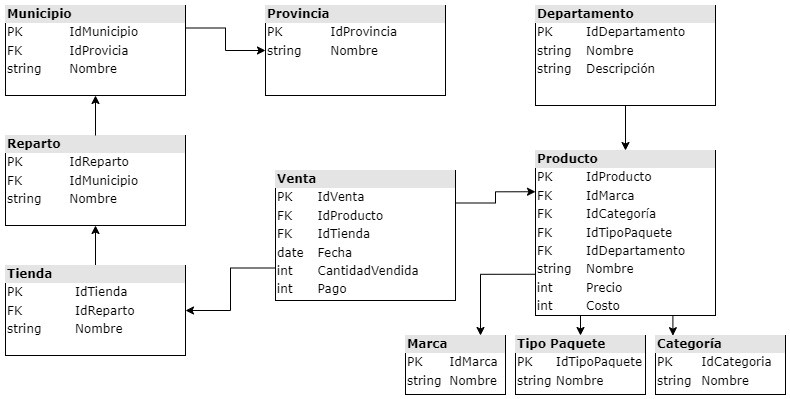
\includegraphics[scale=0.7]{../document/Graphics/retailSales-Transactional.jpg}
    \caption{Sistema Transaccional: Ventas Minoristas}
    \label{fig:retail-transactional}
  \end{figure}

En la carpeta \textbf{Retail\_Sales} se encunetran los scripts de python \textbf{retailSalesDB.py} y \textbf{populateDB.py} 
los cuales se encargan de crear la base de datos y poblarla de valores aleatorios respectivamente. El gestor de bases de 
datos utilizado es PostgreSQL y se utilizó para la comunicación con el mismo el ORM SQLAlchemy de python y el adaptador 
de PostgreSQL para python Psycopg2.

El objetivo del experimento es generar el c\'odigo y pipeline de los procesos ETL necesarios para crear y mantener,
a partir del sistema transaccional de ventas minoristas, un almacén de datos compuesto por las dimensiones Tienda, 
Producto y Fecha, y por la tabla de hechos Venta. La Figura\ref{fig:retail-Warehouse} muestra la composición de las 
tablas de dimensión y de hechos del almacén de datos propuesto.

\begin{figure}
    \centering
    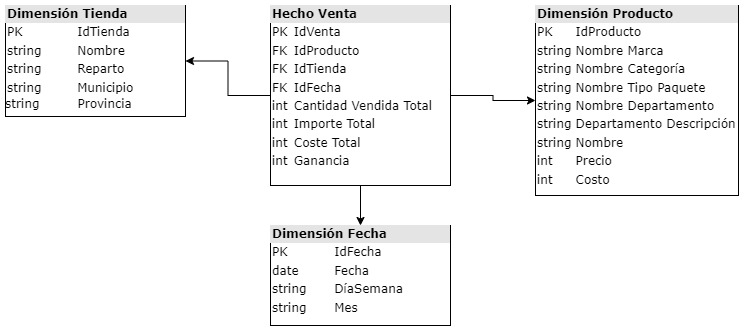
\includegraphics[scale=0.5]{../document/Graphics/retailSales-Data Warehouse.jpg}
    \caption{Almacén de Datos: Ventas Minoristas}
    \label{fig:retail-Warehouse}
  \end{figure}